
\chapter{Implementácia a testovanie}

V tejto kapitole bude opísaná implementácia a rozdelenie komponentov vzhľadom na navrhovaný postup.
Kapitola priblíži počty dát pre trénovanie modelov, tvorbu modelov ich trénovanie, ukladanie a meranie ich úspešnoti.



\section{Trénovacie dáta}
\label{sec:trenovaciedata}

\subsection{Zber dát}
Pre trénovanie modelov boli použité obrázky zo zdrojov spomenutých v kapitole \ref{sec:databaza}.
Tabuľka nižšie uvádza podrobné počty obrázkov z daných zdrojov ktoré boli použité pre určenie typu zbrane v 2 kategóriách.

\begin{table}[H]
  \centering
  \label{my-label}
  \begin{tabular}{|l|c|c|}
    \hline
    Zdroj               & \multicolumn{1}{l|}{Počet krátkych zbraní} & \multicolumn{1}{l|}{Počet dlhých zbraní} \\ \hline
    IMFDB               & 647                                        & 670                                      \\ \hline
    ImageNet            & 730                                        & 94                                       \\ \hline
    Google vyhľadávanie & 0                                          & 86                                       \\ \hline \hline
    SPOLU               & 1377                                       & 850                                      \\ \hline
  \end{tabular}
  \caption{Podrobné počty trénovacích dát.}
\end{table}

Vo všeobecnosti je jednoduchšie nájsť obrázky ktoré obsahujú krátke zbrane (pištole) ako dlhé zbrane.
Databáza ImageNet obsahovala vyše 3000 odkazov na obrázky, avšak veľká časť z nich bola chybná alebo daný súbor už neexistoval.

Ako bolo spomínané v \ref{subsec:generovanie3d}, obrázky ktoré boli použité na trénovanie modelov pre určenie náklonu zbrane bolo potrebné
    vygenerovať pomocou 3D modelov.
Pre toto generovanie bolo použitých desať pozadí scény a päť 3D modelov z toho tri modely boli dlhé zbrane a dve modely krátkych zbraní.

\begin{figure}[H]
    \centering
    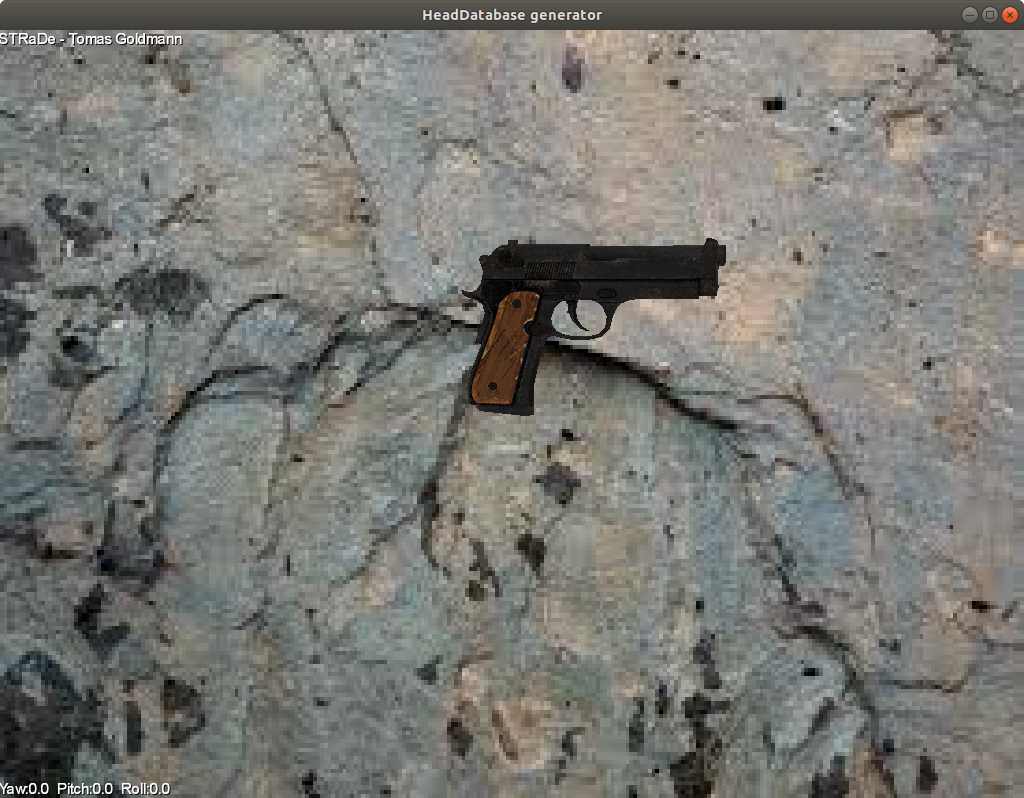
\includegraphics[width=0.7\textwidth]{generator3d}
    \caption{Program pre generovanie obrázkov z 3D modelov.}
    \label{pic:generator3d}
\end{figure}

Niektoré použité modely mali nastavený zlý bod otáčania a taktiež boli veľmi malé.
Preto, ako je vidieť na obrázku \ref{pic:generator3d}, museli byť výsledne obrázky ešte orezané aby sa vnich nachádzala iba zbran bez nepotrebného okolia.

\begin{figure}[H]
    \centering
    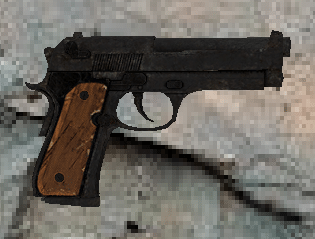
\includegraphics[width=0.5\textwidth]{croped_weapon}
    \caption{Výsledný vygenerovaný obrázok po orezaní okolia.}
    \label{pic:generator3d}
\end{figure}

Tabuľka nižsie uvádza presné počty vygenerovaných obrázkov.

\begin{table}[H]
    \centering
    \label{my-label}
    \begin{tabular}{|l|c|}
        \hline
        Typ osi otáčania & \multicolumn{1}{l|}{Počet obrázkov} \\ \hline
        pitch            & 1480                                \\ \hline
        roll             & 4450                                \\ \hline
        yaw              & 4600                                \\ \hline
        \end{tabular}
    \caption{Podrobné počty trénovacích dát.}
\end{table}

Pre os otáčania pitch boli vybrané obrázky z datasetu určeného pre klasifikáciu typu zbrane.
Pre zvyšné 2 osi boli obrázky generované, počty sa líša kvôli niektorým chybným obrázkom ktoré museli byť vymazané.

\subsection{Načítavanie dát}
\label{subsec:nacitaniedat}
Pre načítavanie dát je implementovaná trieda \textit{DataLoader} v scripte \textit{loader.py}.
Trieda obsahuje niekoľko funkcií pre načítanie týchto dát, tieto funkcie vrátia pole načitaných obrázkov, pole indexov označení [eng. labels] obrázkov a
    štruktúru typu dictionary ktorá obsahuje index a názov označenia, napr. \{0: ``kratka zbran'', 1: ``dlha zbran''\}.

Prvá z funkcií načitáva dáta z priečinka kde označenie obrázkov, či je to krátka alebo dlhá zbraň, je zabezpečené podľa názvou podpriečinkou.
Pre obrázky o náklne zbrane sa označenie osi berie takisto z názvu podpriečinka, avšak presné označenie o koľko stupňov je model v obrázku otočený
    je získaný z názvu obrázka ktorý musí spĺnať presný formát: \textit{p0.0\_y0.0\_r0.0-typzbrane.jpg}.
Kde \textit{p0.0} označuje hodnotu náklonu v osi pitch, \textit{y0.0} hodnotu náklonu v osi yaw, \textit{r0.0} v osi roll a \textit{typzbrane} môže byť
    akýkoľvek reťazec.
Formát vstupných obrázkov môže byť \textit{.jpg} alebo \textit{.jpeg}.

Správnu hierarchiu priečinkou je vidieť na obrázoku \ref{pic:folderhierarchy}

\begin{figure}[H]
    \centering
    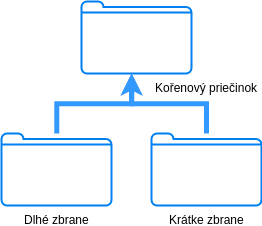
\includegraphics[width=0.32\textwidth]{class_hierarchy}
    \qquad
    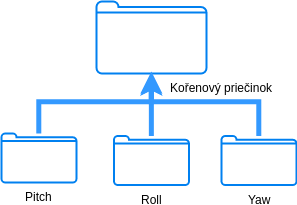
\includegraphics[width=0.4\textwidth]{angle_hierarchy}
    \caption{Hierarchia priečinkou pre správne označenie vstupných obrázkov.}
    \label{pic:folderhierarchy}
\end{figure}

Druhá z funkcií umožňuje načítať zoznam obrázkov z textového súboru, kde sa na každom riadku nachádza práve jedna cesta k požadovanému obrázku.
Spôspob označovania obrázkov je rovnaký ako v prvom prípade, preto je taktiež potrebné dodržat správnu hierachiu priečinkou.

\subsection{Predspracovanie dát}
\label{subsec:predspracovaniedat}
Pre predspracovanie obrazu sú implementované 2 triedy \textit{Preprocessor} a \textit{Preprocessing} v scripte \textit{preprocessing.py}.
Trieda \textit{Preprocessor} obsahuje list do ktorého je možné pridávať funckíe ktoré sú implementované v triede \textit{Preprocessing}.
Po zavolaní funkcie \textit{apply(input\_data)} z triedy \textit{Preprocessor}, sa tieto
    funkcie v poradí v akom boli pridané do listu zavolajú a prebehne predspracovanie vstupných dát.
Každá z možností predspracovanie obrazu ktorá bola uvedená v \ref{sec:preprocessing}, je implementovaná v triede \textit{Preprocessing} pomocou
    knižnice scikit-image.

Pre augmentáciu dát určených na klasfikáciu typu zbrane je použitá trieda \textit{ImageDataGenerator} z knižnice Keras.
Parametre tohto generátora sú nastavená na: horizonálne a vertikálne preklopenia obrázka, posun obrázka až o 15\% jeho dĺžky alebo šírky,
    rotácia o náhodný uhol v rozsahu 0 až 180 stupňov a doplnenie čiernych pixelov pomocou nastavenia ``nearest''.

Pre augmentáciu dát pre určenie náklonu zbrane je implementovaná samostatná trieda \textit{AngleGenerator}, ktorá zabezpečuje správne dogenerovanie
    vstupných dát pomocou horizontálneho alebo vertikálneho preklopenia obrázka a správneho výpočtu uhlu natočenia (viď. \ref{subsec:augmentacia}).



\section{Modely}
\label{sec:modely}
Všetky modely pre trénovanie su implementované v scripte \textit{models.py}.
Existuje jedna hlavná trieda \textit{class Model}, ktorá obsahuje všetky základne atributy potrebné pre modely, ako npr.
    meno modelu, vstupný rozmer dát, zvolený algoritmus trénovania a štruktúru typu dictionary ktorá obsahuje indexi a názvi označení obrázkov.

Každý model následne dedí z tejto hlavnej triedy a implementuje v sebe 2 funkcie \textit{build} ktorá zabezpečuje vytvorenie modelu a
    funkciu \textit{train} ktorá sa volá pri spustení trénovania daného modelu.

\begin{figure}[H]
    \centering
    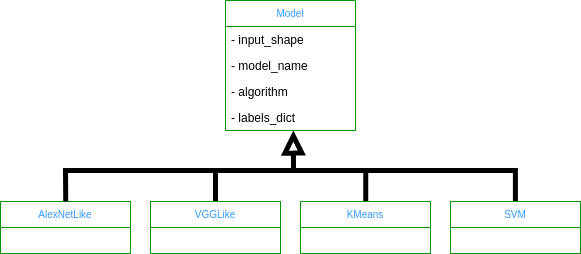
\includegraphics[width=0.8\textwidth]{inheritance}
    \caption{Hierarchia dedenia tried modelov.}
    \label{pic:inheritance}
\end{figure}

Konvolučné neurónové siete su implementované pomocou triedy \textit{Sequencia} z knižnice Keras.
Pre klasifikátor K-Nearest-Neighbor je použitá trieda \textit{KNeighborsClassifier} a trieda \textit{SVC} pre klasifikátor SVM z knižnice scikit-learn.
%Pre klasifikátor K-Nearest-Neighbor je použitá trieda \textit{KNeighborsClassifier} s počtom 1 a 5 najbližších susedov, a trieda \textit{SVC} pre klasifikátor SVM
%    so základnymi nastavenia trénovania z knižnice scikit-learn.

\subsection{Ukladanie a načitanie modelu}
\label{subsec:ukladaniemodelu}
Pre ukladanie natrénovaných modelov je implemtovaná funkcia \textit{save\_model()} v triede \textit{DataSaver} v scripte \textit{loader.py}.
Pri ukladaní modelu sa ukladá model v binárnej forme, ukladá sa konfiguračný súbor \textit{settings.json} ktorý obsahuje informácie ako veľkosť
    vstupných dát, použité funkcie na predspracovanie dát, meno modelu, typ algoritmu učenia, zoznam indexov označenia dát a dalšie informácie
    špecifické pre daný typ modelu.
Uložením konvolučnéj neurónovej siete sa ukladá graf priebehu trénovanie.

Naopak pre načitanie modelov je implementovaná funkcia \textit{load\_model\_data()} v triede \textit{DataLoader} v scripte \textit{loader.py},
    ktorá načíta binárnu podobu modelu a všetky informácie z konfiguračného súboru \textit{settings.json}.



\section{Testovanie}
\label{sec:testovanie}
Pre testovanie riešenia tejto práce sa využíva funkcia zodpovedná za evaluáciu modelov \textit{evaluate\_model} v scripte \textit{evaluation.py}
    podľa metrík ktoré boli spomenuté už vyššie.
Testovanie modelov prebieha ako určovanie presnosti týchto natrénovaných modelov.

\begin{figure}[H]
    \centering
    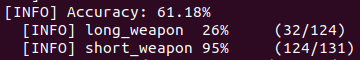
\includegraphics[width=0.75\textwidth]{testovanie}
    \caption{Príklad výstupu po testovaní modelu určujúceho typ zbrane.}
    \label{pic:testovanie}
\end{figure}

\begin{figure}[H]
    \centering
    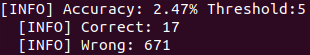
\includegraphics[width=0.7\textwidth]{testovanie_angle}
    \caption{Príklad výstupu po testovaní modelu určujúceho náklon zbrane.}
    \label{pic:testovanie}
\end{figure}



\section{Záver implementácie}

Kapitola v úvode uvádza presné počty dát, podľa zdrojov, ktoré sú použité pre tŕenovanie modelov.
Vysvetľuje postup generovania obrázkov z 3D modelov.
Ďalej sa venuje možnostiam načítavania dát zo súboru alebo priečinkov pri dodržaní potrebnej hierarchie priečinkov a názvov súborov.
Približuje triedy, ktoré implementujú predspracovanie vstupných dát, tvorbu modelov, uvádza informácie, ktoré sú uložené
    pri ukladaní modelov a spôsob ich načítania.
Nasleduje celý postup trénovania modelov, opis scriptu, ktorý toto trénovanie uľahčuje a vysvetľuje metriky, podľa ktorých sa hodnotí presnosť modelov.
